\documentclass[12pt,a4paper]{report}

% ── Core layout ──────────────────────────────────────────────
\usepackage[top=1in,bottom=1in,left=1.25in,right=1in]{geometry}
\usepackage{setspace}
\usepackage{graphicx}
\usepackage{float}
\usepackage{placeins}       % \FloatBarrier keeps figures in their section
\usepackage{booktabs}
\usepackage{array}
\usepackage{tabularx}       % auto-stretch columns; avoids overflow
\usepackage{adjustbox}      % safety net: shrinks any table that still overflows
\usepackage{enumitem}
\usepackage{hyperref}
\usepackage{xcolor}
\usepackage{longtable}
\usepackage{titlesec}
\usepackage{caption}
\usepackage{fancyhdr}
\usepackage{parskip}        % space between paragraphs instead of indent
\usepackage{microtype}      % better line-breaking / justification
\usepackage{ragged2e}

% ── Fix fancyhdr headheight warning ──────────────────────────
\setlength{\headheight}{14.5pt}
\addtolength{\topmargin}{-2.5pt}

% ── Ragged-right column type for tables (kills Underfull) ────
\newcolumntype{L}[1]{>{\RaggedRight\arraybackslash}p{#1}}

\hypersetup{
  colorlinks=true,
  linkcolor=blue,
  urlcolor=blue,
  citecolor=blue
}

\setstretch{1.25}
\setlength{\emergencystretch}{3em}   % allows extra stretch before Overfull fires
\setlist[itemize]{noitemsep, topsep=4pt}
\setlist[enumerate]{noitemsep, topsep=4pt}

% ── Header / footer ──────────────────────────────────────────
\pagestyle{fancy}
\fancyhf{}
\rhead{StyleSense AI}
\lhead{Project Report}
\cfoot{\thepage}
\renewcommand{\headrulewidth}{0.4pt}

% ── Chapter title style ──────────────────────────────────────
\titleformat{\chapter}[display]
  {\normalfont\bfseries\LARGE}{CHAPTER \thechapter.}{10pt}{\LARGE}
\titlespacing*{\chapter}{0pt}{20pt}{20pt}

% ── Consistent table spacing ─────────────────────────────────
\setlength{\tabcolsep}{7pt}
\renewcommand{\arraystretch}{1.3}

% ── Project metadata (edit these values) ─────────────────────
\newcommand{\ProjectTitle}{StyleSense AI: An Intelligent Mobile System for
  Personalized Fashion Recommendation and Virtual Try-On}
\newcommand{\ProjectShort}{StyleSense AI}
\newcommand{\TeamA}{JAPJIT}
\newcommand{\TeamB}{PRABHSIMRAN}
\newcommand{\TeamC}{PANSHUL}
\newcommand{\TeamD}{RATIK}
\newcommand{\TeamE}{ABHINEET}
\newcommand{\CourseName}{Minor Project}
\newcommand{\InstituteName}{(Your Institute Name)}
\newcommand{\DepartmentName}{(Your Department)}
\newcommand{\SubmissionMonthYear}{April 2026}

% ── Helpers ──────────────────────────────────────────────────
% A table that auto-fits within the text column
\newenvironment{fitstable}[1][htbp]{%
  \begin{table}[#1]\centering%
  \adjustbox{max width=\linewidth}{%
}{%
  }\end{table}%
}

\begin{document}

% =========================================================
% TITLE PAGE
% =========================================================
\begin{titlepage}
  \centering
  \vspace*{1.2cm}
  {\Large \textbf{\InstituteName} \par}
  \vspace{0.3cm}
  {\large \DepartmentName \par}
  \vspace{1.2cm}
  \rule{\textwidth}{1.5pt}\par
  \vspace{0.4cm}
  {\Huge\bfseries \ProjectTitle \par}
  \vspace{0.4cm}
  \rule{\textwidth}{1.5pt}\par
  \vspace{0.8cm}
  {\large \textit{A \CourseName{} Report} \par}
  \vspace{1.4cm}

  \begin{tabular}{rl}
    \textbf{Team Members:} & \TeamA \\
                           & \TeamB \\
                           & \TeamC \\
                           & \TeamD \\
                           & \TeamE \\
  \end{tabular}

  \vfill
  {\large \SubmissionMonthYear \par}
\end{titlepage}

% =========================================================
% ABSTRACT
% =========================================================
\pagenumbering{roman}
\chapter*{ABSTRACT}
\addcontentsline{toc}{chapter}{ABSTRACT}

Modern fashion e-commerce overwhelms users with thousands of product choices while simultaneously offering very little context-aware personalization. Recommendation engines on mainstream platforms ignore critical user signals such as body type, skin tone, local weather, budget, and the items a user already owns. As a result, users experience decision fatigue and frequently return purchased items.

\textbf{\ProjectShort{}} addresses these problems through a two-tier system: an Android mobile application (built with Kotlin and Jetpack Compose) paired with a Python FastAPI backend. The backend scrapes live product listings from Myntra, scores candidates using a multi-factor \textit{MatchScorer} engine that weighs style, color, brand, weather, and user feedback, and caches results efficiently in Redis. For users who want to see how a garment looks on them before buying, the system integrates a \textit{virtual try-on} feature that proxies a hosted AI model on Hugging Face Spaces via the Gradio API, returning a generated image directly to the app.

User identity and profile data (collected through a 10-step onboarding flow) are persisted in Firebase Firestore. Weather-aware suggestions are powered by the OpenWeatherMap API using the device's GPS coordinates.

This report documents the project motivation, a review of relevant literature, the complete design flow and module architecture, implementation results for each module, and future directions such as expanding to multi-store scraping and learning-based ranking.

\tableofcontents
\listoffigures
\listoftables

% =========================================================
% LIST OF STANDARDS
% =========================================================
\chapter*{LIST OF STANDARDS}
\addcontentsline{toc}{chapter}{LIST OF STANDARDS}

\textit{The following standards and guidelines were used as references during the design and implementation of \ProjectShort{}. They are cited here to demonstrate that engineering and security best practices were considered.}

\vspace{8pt}
\begin{adjustbox}{max width=\linewidth}
\begin{tabular}{L{0.28\linewidth} L{0.66\linewidth}}
\toprule
\textbf{Standard / Guideline} & \textbf{Where and Why Used in \ProjectShort{}} \\
\midrule
OWASP Mobile Security Testing Guide (MSTG)
  & Used as a security checklist for the Android app: secure token storage,
    certificate validation, network communication, and authentication flow. \\
OAuth 2.0 / OpenID Connect
  & Authentication protocol underlying Firebase Google Sign-In via the
    Android Credential Manager. \\
RESTful API Design Principles
  & Backend endpoints follow predictable HTTP method + versioned path
    conventions (\texttt{/api/v1/...}) with JSON and multipart payloads. \\
IEEE 29148 (Systems and Software Engineering --- Requirements)
  & Used as a structural reference for requirement identification, decomposition
    into tasks, and mapping to features. \\
Material Design 3 (Google)
  & UI component guidelines and interaction patterns applied through
    Jetpack Compose and the Material 3 library. \\
\bottomrule
\end{tabular}
\end{adjustbox}

\clearpage
\pagenumbering{arabic}

% =========================================================
% CHAPTER 1 — INTRODUCTION
% =========================================================
\chapter{INTRODUCTION}

\textit{This chapter introduces the context and motivation for \ProjectShort{}, formally states the problem, describes the tasks undertaken, and provides a timeline and organization of the rest of the report.}

\section{Identification of Client / Need / Relevant Contemporary Issue}

\textbf{Who is the client?} The end-user of \ProjectShort{} is any online fashion shopper in India who browses e-commerce platforms such as Myntra, AJIO, or Amazon Fashion. According to industry estimates, India's fashion e-commerce segment is one of the fastest-growing in the world, with hundreds of millions of active shoppers and thousands of new products listed every day.

\textbf{What is the contemporary need?} Despite the large catalogs available online, users frequently report:
\begin{itemize}
  \item \textbf{Decision fatigue} --- too many choices, too little guidance.
  \item \textbf{Poor fit and appearance confidence} --- users cannot visualize whether a garment suits their body type, skin tone, or existing wardrobe.
  \item \textbf{Context blindness} --- recommendations do not adapt to occasion (e.g., office, wedding, casual), weather conditions, or the user's own closet.
\end{itemize}

These issues collectively lead to high purchase-return rates (industry estimates suggest 20--35\% of online fashion orders are returned), which is costly for both consumers and retailers.

\section{Identification of Problem}

Most recommendation systems on fashion platforms rely primarily on \textit{purchase history} and \textit{popularity scores}. This creates a severe \textbf{cold-start problem}: new users who have no purchase history receive irrelevant generic suggestions. Furthermore, even for returning users, the recommendations rarely factor in:
\begin{itemize}
  \item Body type and size/measurements.
  \item Skin tone (relevant for color matching).
  \item Local weather at the time of browsing.
  \item Occasion or dress code constraints.
  \item Compatibility with clothing the user already owns.
\end{itemize}
Additionally, virtual try-on --- the ability to preview how a garment looks on the user's own body --- is either absent or available only as an isolated feature disconnected from the recommendation flow.

\textbf{Problem statement:} \textit{Design and implement a mobile application that provides context-aware, profile-driven fashion recommendations from live e-commerce data, and integrates AI-based virtual try-on to help users make confident purchase decisions.}

\section{Identification of Tasks}

The following modules/tasks were identified and assigned to team members:

\begin{itemize}
  \item \textbf{Mobile Application (Android):} Design and build all UI screens using Jetpack Compose and Navigation Compose, including authentication, onboarding, home, wardrobe, recommendations, saved items, try-on, and settings. Implement ViewModels and repositories to manage state and data flow.
  \item \textbf{Backend API (FastAPI):} Implement a Python FastAPI server with endpoints for recommendations, feedback, saved items, wardrobe image upload, scraper connectivity check, and virtual try-on proxy. Handle request validation, caching, and error handling.
  \item \textbf{Data Collection (Scraping):} Build a web scraper for Myntra product listing pages that generates stable queries from user profiles, parses product data, and normalizes fields into the backend's data model.
  \item \textbf{Recommendation Engine:} Implement the \texttt{MatchScorer} ranking component that scores each candidate product using style, color, brand, weather, and feedback signals. Implement result diversification and stable pagination.
  \item \textbf{Storage and Caching:} Integrate Firebase Auth (Google Sign-In), Firestore for user profiles and wardrobe metadata, and Redis for caching scraped candidates, ranked lists, and feedback sets.
  \item \textbf{Virtual Try-On:} Build the try-on proxy that downloads garment images, normalizes inputs, calls a hosted Hugging Face Gradio Space, and returns a generated try-on image as base64 to the app.
\end{itemize}

\section{Timeline}

Table~\ref{tab:timeline} shows the planned schedule across a 12-week minor project period. Each pair of weeks corresponds to a major deliverable.

\vspace{4pt}
\begin{table}[H]
\centering
\caption{Project Development Timeline}
\label{tab:timeline}
\begin{adjustbox}{max width=\linewidth}
\begin{tabular}{L{0.13\linewidth} L{0.81\linewidth}}
\toprule
\textbf{Weeks} & \textbf{Planned Activities and Deliverables} \\
\midrule
1--2  & Requirements analysis, module decomposition, toolchain setup (Android Studio,
        Python virtual env, Firebase project, Redis local install). \\
3--4  & Android UI scaffolding: navigation graph, splash/sign-in/onboarding screen skeletons,
        profile data models, Firestore schema design. \\
5--6  & FastAPI backend skeleton: all endpoint stubs, Pydantic models for request/response,
        Retrofit client on Android, wardrobe upload endpoint (end-to-end tested). \\
7--8  & Myntra scraper implementation (query building, HTML parsing, candidate normalization);
        MatchScorer ranking logic; Redis caching and pagination. \\
9--10 & Virtual try-on integration (Gradio client, fallback handling, base64 return);
        Firebase Auth + Firestore profile read/write; feedback + saved items flow. \\
11--12 & Integration testing across all modules, UI polish, performance checks,
         documentation, and report preparation. \\
\bottomrule
\end{tabular}
\end{adjustbox}
\end{table}

\section{Organization of the Report}

\textbf{Chapter 1 (Introduction)} introduces the motivation, problem statement, task breakdown, and timeline. \textbf{Chapter 2 (Literature Review)} surveys existing work in fashion recommendation, virtual try-on, and context-aware systems, and presents a bibliometric analysis of key research papers. \textbf{Chapter 3 (Design Flow/Process)} covers specifications, constraints, module architecture, technology selection decisions, and the implementation methodology. \textbf{Chapter 4 (Results Analysis and Validation)} demonstrates each module's implementation and summarizes endpoint-level validation. \textbf{Chapter 5 (Conclusion and Future Work)} summarizes achievements and proposes improvements. References, appendices (design checklist, plagiarism report), and a user manual follow at the end.

% =========================================================
% CHAPTER 2 — LITERATURE REVIEW
% =========================================================
\chapter{LITERATURE REVIEW / BACKGROUND STUDY}

\textit{This chapter traces the evolution of fashion recommendation and virtual try-on research, examines existing commercial solutions, performs a bibliometric analysis of the most relevant academic papers, and derives the research gap that \ProjectShort{} addresses. It concludes with a formal problem definition and project objectives.}

\section{Timeline of the Reported Problem}

The problem of helping consumers choose clothing has existed since catalogue shopping in the early 20th century. The computational version of this problem has evolved in four distinct phases:

\begin{enumerate}
  \item \textbf{Content-Based Filtering (1990s--2000s):} Early digital recommendation systems matched items by explicit attributes such as category, colour keywords, and price range. Personalization was limited to rule-based filters set by the user themselves.
  \item \textbf{Collaborative Filtering (2000s--2010s):} Systems like Amazon's item-based collaborative filtering (Linden et al., 2003) inferred preferences from collective user-item interactions. These systems required substantial purchase history, creating a cold-start problem for new users.
  \item \textbf{Deep Learning and Visual Fashion AI (2014--2020):} The release of large annotated fashion datasets (e.g., DeepFashion, Liu et al., 2016) enabled deep learning models to understand visual semantics of clothing --- style, silhouette, pattern, and colour --- and perform similarity-based retrieval. Convolutional neural networks (He et al., 2016) became standard visual encoders. Virtual try-on research also emerged during this period (Han et al., 2018 VITON), using image warping networks to composite garments onto user photos.
  \item \textbf{Multimodal and Context-Aware Systems (2020--present):} Recent systems combine text, image, and contextual signals (time of day, weather, social occasion). Transformer-based models and large language models are increasingly used for outfit generation and personalized styling dialogue. Virtual try-on quality improved dramatically with diffusion-based models (IDM-VTON, 2023+).
\end{enumerate}

Despite this progress, most \textit{commercial} applications available to Indian consumers still lag in context-awareness and do not offer profile-driven personalization that factors in body type, skin tone, wardrobe compatibility, and live weather together.

\section{Existing Solutions}

\textit{This section surveys existing products that partially address the problem and identifies the gap that \ProjectShort{} fills.}

Table~\ref{tab:existing} compares five representative systems across key personalization dimensions. The last row shows \ProjectShort{}'s positioning.

\vspace{4pt}
\begin{table}[H]
\centering
\caption{Comparison of Existing Fashion Recommendation Approaches}
\label{tab:existing}
\begin{adjustbox}{max width=\linewidth}
\begin{tabular}{L{0.15\linewidth} L{0.12\linewidth} L{0.12\linewidth} L{0.12\linewidth} L{0.12\linewidth} L{0.28\linewidth}}
\toprule
\textbf{System} & \textbf{Body Type Aware} & \textbf{Weather Aware} & \textbf{Wardrobe Aware} & \textbf{Virtual Try-On} & \textbf{Key Limitation} \\
\midrule
Myntra (App)      & Partial & No  & No  & Limited & Popularity-driven; no wardrobe or weather context. \\
ASOS              & Size guide & No & No & No & No contextual or wardrobe adaptation. \\
Stitch Fix        & Yes & No & Partial & No & Subscription + human stylist; US-only; no live browsing. \\
H\&M Style Quiz   & Partial & No & No & No & Static quiz; not connected to live dynamic catalog. \\
Google Lens       & No & No & No & No & Visual search only; not a personalized recommender. \\
\midrule
\textbf{\ProjectShort{}} & \textbf{Yes} & \textbf{Yes} & \textbf{Yes} & \textbf{Yes} & Scraping-dependent; try-on latency from hosted model. \\
\bottomrule
\end{tabular}
\end{adjustbox}
\end{table}

As seen in Table~\ref{tab:existing}, no single existing solution combines all five personalization dimensions. \ProjectShort{} is designed to address this gap within the constraints of a minor project (no GPU infrastructure, no large training dataset).

\section{Bibliometric Analysis}

\subsection*{What is Bibliometric Analysis?}

\textbf{Bibliometric analysis} is a \textit{quantitative, systematic method} for evaluating and mapping a body of research literature. Unlike a traditional narrative literature review (which simply summarises papers the author selected), a bibliometric analysis uses \textit{measurable indicators} to characterise the state of a research field. Common indicators include:

\begin{itemize}
  \item \textbf{Publication volume over time} --- how many papers appear per year, showing whether interest is growing or declining.
  \item \textbf{Citation counts} --- which works are most influential.
  \item \textbf{Keyword co-occurrence} --- which topics cluster together (e.g., ``fashion'' + ``deep learning'' + ``try-on'').
  \item \textbf{Author/venue distribution} --- which research groups and conferences lead the field.
\end{itemize}

\textbf{Why is it included in an engineering project report?} In a design-oriented report, bibliometric analysis serves two purposes:
\begin{enumerate}
  \item It demonstrates that the chosen approach is \textit{grounded in existing research} and not invented in isolation.
  \item It provides an \textit{objective justification} for design decisions (e.g., ``the literature shows rule-based scoring is practical for cold-start; that is why we use MatchScorer instead of a neural ranker'').
\end{enumerate}

\subsection*{Methodology Applied Here}

For this project, the literature was searched using Google Scholar and ACM Digital Library using the following keyword clusters: \textit{fashion recommendation system}, \textit{virtual try-on network}, \textit{context-aware recommender system}, \textit{outfit compatibility}, and \textit{body-type clothing suggestion}. Papers were filtered to those with more than 100 citations or published in top venues (CVPR, ECCV, ACM RecSys). The result is six representative works, summarised in Table~\ref{tab:papers} and discussed below.

\vspace{4pt}
\begin{table}[H]
\centering
\caption{Bibliometric Summary of Key Related Works}
\label{tab:papers}
\begin{adjustbox}{max width=\linewidth}
\begin{tabular}{L{0.20\linewidth} L{0.07\linewidth} L{0.20\linewidth} L{0.20\linewidth} L{0.24\linewidth}}
\toprule
\textbf{Paper / Authors} & \textbf{Year} & \textbf{Research Topic} & \textbf{Key Contribution} & \textbf{Relevance to \ProjectShort{}} \\
\midrule
DeepFashion (Liu et al.)
  & 2016
  & Fashion image recognition and retrieval
  & Large-scale annotated dataset (800K images); enables training clothing classifiers
  & Motivates image-driven category/style understanding \\
ResNet (He et al.)
  & 2016
  & Deep residual visual learning
  & Residual connections enabling very deep CNNs; standard visual feature extractor
  & Underpins modern fashion embedding models \\
VITON (Han et al.)
  & 2018
  & Virtual try-on
  & Image-based try-on via shape and appearance warping; composites garment onto user photo
  & Directly motivates our try-on module; IDM-VTON is a descendant \\
Context-Aware Recommenders (Adomavicius \& Tuzhilin)
  & 2011
  & Recommender system survey
  & Formalises contextual information (time, location, weather) in recommendation models
  & Justifies incorporating weather and occasion signals \\
Outfit Compatibility (Cheng et al.)
  & 2021
  & Outfit generation and compatibility
  & Models inter-item compatibility beyond single-item relevance
  & Motivates wardrobe-aware recommendations \\
Body-type Styling (domain studies)
  & Various
  & Fit/body-type fashion guidance
  & Shows body shape and measurements materially affect garment suitability
  & Motivates collecting body type and measurements during onboarding \\
\bottomrule
\end{tabular}
\end{adjustbox}
\end{table}

\subsection*{Discussion of Individual Works}

\textbf{DeepFashion (Liu et al., 2016)} introduced one of the first large-scale annotated fashion datasets comprising over 800,000 images with rich attribute labels (category, colour, pattern, occasion). This work demonstrated that deep convolutional networks can reliably classify and retrieve fashion items. It motivates our use of product images and category/style metadata as primary features in the MatchScorer.

\textbf{Deep Residual Networks (He et al., 2016)} proposed the residual learning framework, allowing training of networks with hundreds of layers. ResNet variants became the de facto visual feature extractor for fashion tasks. This work is cited because any modern fashion embedding pipeline (including those underlying the Hugging Face try-on Space we use) builds on this foundation.

\textbf{VITON (Han et al., 2018)} was the first end-to-end image-based virtual try-on network that generates a photorealistic image of a person wearing a given garment. It works by learning to warp the cloth shape to the target pose and blend it with the person image. This directly motivates our try-on module. The Hugging Face Space used in \ProjectShort{} (IDM-VTON) is a more recent descendant using diffusion-based generation, which produces more realistic results.

\textbf{Context-Aware Recommender Systems (Adomavicius \& Tuzhilin, 2011)} provides the theoretical framework for incorporating contextual information --- time, location, weather, companion, activity --- into recommendation models. Their multi-dimensional model formalises why weather and occasion should be first-class signals in a fashion recommender, not afterthoughts. This justifies our MatchScorer's weather adjustment and the occasion/dress-code fields collected on the Home screen.

\textbf{Outfit Compatibility (Cheng et al., 2021)} demonstrates that fashion recommendation should not treat each item in isolation. Compatible items (those that ``go together'' visually and stylistically) form outfits, and recommending items that complement what a user already owns leads to higher satisfaction. This motivates the wardrobe upload feature and the wardrobe-aware weighting in MatchScorer.

\textbf{Body-type and Fit Studies} from fashion design and consumer behaviour research consistently show that garment suitability depends significantly on the wearer's body shape and measurements. This justifies collecting body type (e.g., ectomorph/mesomorph/endomorph or hourglass/pear/rectangle) and size measurements during onboarding, and using them as constraints in the MatchScorer.

\section{Review Summary}

\textit{This section consolidates what the literature tells us and shows how it directly shaped design decisions in \ProjectShort{}.}

\begin{enumerate}
  \item \textbf{Cold-start needs profile-driven rules.} Collaborative filtering requires purchase
        history. For new users a rule-based scorer using explicit attributes (body type, style,
        budget) is more effective --- this is why \texttt{MatchScorer} uses feature matching
        rather than learned embeddings.
  \item \textbf{Virtual try-on is compute-heavy; use a hosted model.} VITON-style models
        require GPU inference. Proxying a hosted Hugging Face Space is the practical
        solution for a minor project with no dedicated GPU.
  \item \textbf{Weather and occasion are strong personalization signals.} Context-aware
        recommender research confirms that adding weather and activity context improves
        satisfaction, justifying the OpenWeatherMap integration and the Home-screen
        occasion/dress-code fields.
  \item \textbf{Wardrobe compatibility is commercially underexplored.} Despite research on
        outfit compatibility, most apps ignore the user's existing wardrobe --- making
        this a key differentiating feature of \ProjectShort{}.
\end{enumerate}

\section{Problem Definition}

Based on the gaps identified in the literature review, the following formal problem statement guides this project:

\begin{quote}
\textit{Design and implement a full-stack mobile application that retrieves live fashion
product candidates from an e-commerce source, ranks them using a multi-factor scoring
model that incorporates user profile signals (body type, skin tone, size, style preference,
budget), contextual inputs (occasion, dress code, weather condition), and wardrobe
inventory, and offers a virtual try-on preview by invoking a hosted AI image generation
model --- all within the constraints of a minor project (no on-device ML training,
no dedicated GPU).}
\end{quote}

\section{Goals / Objectives}

The following SMART (Specific, Measurable, Achievable, Relevant, Time-bound) objectives govern the project:

\begin{enumerate}
  \item Collect a comprehensive user profile through a 10-step onboarding flow and persist it securely in Firestore.
  \item Provide paginated, real-world product recommendations by scraping Myntra and returning ranked results with explanatory match reasons.
  \item Incorporate wardrobe signals so that recommended items complement clothing the user already owns.
  \item Integrate weather-aware scoring by fetching live weather data from OpenWeatherMap using the device's GPS coordinates.
  \item Capture like/dislike feedback per recommendation and reflect it in subsequent re-rankings without additional user input.
  \item Provide a virtual try-on preview for any selected garment by invoking a hosted AI model, displaying the generated image and saving it to a local history.
\end{enumerate}

% =========================================================
% CHAPTER 3 — DESIGN FLOW / PROCESS
% =========================================================
\chapter{DESIGN FLOW / PROCESS}

\textit{This chapter documents how the system was designed: which technologies were selected and why, what constraints shaped the design, how individual modules connect, and what implementation methodology was followed. It serves as the engineering rationale for every major decision made in \ProjectShort{}.}

\section{Evaluation and Selection of Specifications / Features}

\textit{Before writing any code, technology choices were evaluated against project constraints (time, compute, cost). Table~\ref{tab:specs} shows the selected stack with brief justification.}

\vspace{4pt}
\begin{table}[H]
\centering
\caption{Technology Specifications and Selection Rationale}
\label{tab:specs}
\begin{adjustbox}{max width=\linewidth}
\small\begin{tabular}{L{0.20\linewidth} L{0.29\linewidth} L{0.42\linewidth}}
\toprule
\textbf{Component} & \textbf{Selected Technology} & \textbf{Why Selected} \\
\midrule
Mobile platform
  & Kotlin + Jetpack Compose (Material 3), Navigation Compose, ViewModel + Coroutines
  & Modern declarative UI; official Google recommendation; state-driven eliminates XML boilerplate. \\
Authentication
  & Firebase Auth (Google Sign-In via Android Credential Manager)
  & No custom auth server needed; Google identity is widely trusted; UID used as primary key everywhere. \\
User / wardrobe database
  & Cloud Firestore
  & Serverless, real-time, free-tier suitable for minor project; automatic offline sync; JSON documents map directly to Kotlin data classes. \\
Backend framework
  & Python FastAPI + Uvicorn
  & Async by default (important for concurrent scraping); auto-generated OpenAPI docs; Pydantic validation reduces bugs. \\
Caching layer
  & Redis (with in-memory fallback)
  & Sub-millisecond read/write; ideal for storing 200-item ranked lists and small feedback sets; fallback ensures resilience. \\
Data collection
  & Web scraping (BeautifulSoup + curl\_cffi)
  & No official public product API available; curl\_cffi mimics real browser fingerprint to reduce blocking. \\
Weather service
  & OpenWeatherMap REST API
  & Free tier supports project scale; returns structured JSON with temperature and weather conditions. \\
Try-on AI
  & Hugging Face Space (IDM-VTON via Gradio client)
  & Eliminates need for GPU server; Gradio client hides API complexity; base64 return avoids file hosting. \\
\bottomrule
\end{tabular}
\end{adjustbox}
\end{table}

\section{Design Constraints}

\textit{Every project operates under constraints. Acknowledging them honestly is good engineering practice --- it shows why certain simplifications were made and where future work should focus.}

\begin{itemize}
  \item \textbf{Compute:} No GPU is available for on-device or self-hosted ML inference. Try-on must use a hosted model; ranking must use rule-based scoring.
  \item \textbf{Scraping reliability:} E-commerce websites can change their HTML structure or block automated requests. This means scraper output is not guaranteed; caching and fallback responses are essential.
  \item \textbf{Try-on latency:} Hugging Face Spaces on free tier can take 20--60 seconds for inference (cold start). The app must show loading state and allow the user to proceed while waiting.
  \item \textbf{Cold-start data:} New users have no purchase history. The system must personalise from explicit signals (onboarding profile) alone.
  \item \textbf{Infrastructure:} Redis is optional; the backend must fall back to in-memory caching if Redis is unavailable to keep the demo functional.
  \item \textbf{Budget:} The project uses free tiers of Firebase, OpenWeatherMap, and Hugging Face. Rate limits apply.
\end{itemize}

\section{Analysis of Features and Finalization Subject to Constraints}

\textit{This section shows how each feature was evaluated against the constraints above and what final design decision was reached. This is the ``why'' behind each implementation choice.}

\vspace{4pt}
\begin{table}[H]
\centering
\caption{Feature Finalization Under Constraints}
\label{tab:finalize}
\begin{adjustbox}{max width=\linewidth}
\small\begin{tabular}{L{0.19\linewidth} L{0.27\linewidth} L{0.21\linewidth} L{0.25\linewidth}}
\toprule
\textbf{Feature} & \textbf{Constraint} & \textbf{Options Considered} & \textbf{Final Decision} \\
\midrule
Product ranking
  & Cold-start; no training data; no GPU
  & Neural ranking, collaborative filtering, rule-based scorer
  & Rule-based MatchScorer: fast, explainable, no training data required. \\
Virtual try-on
  & GPU compute needed; budget \$0
  & Self-hosted model, cloud API, hosted Space
  & Hugging Face Space via Gradio client; free-tier GPU inference. \\
Wardrobe image storage
  & Firestore is not a file store; Firebase Storage adds complexity
  & Firebase Storage, backend static, external CDN
  & Backend static upload (\texttt{/uploads}); URL stored in Firestore. \\
Fast ``Load More''
  & Scraping is slow (2--5 s per query)
  & Re-scrape every time, client-side cache, server-side cache
  & Redis-cached candidate list; re-rank only when feedback version changes. \\
Weather context
  & Requires GPS permission + external API
  & Skip, manual city input, automatic GPS
  & Automatic GPS via Android Location API; backend calls OpenWeatherMap. \\
Authentication
  & Cannot run a custom auth server in minor project timeline
  & Custom JWT, Firebase, Supabase
  & Firebase Auth (Google Sign-In): fully managed, free, secure. \\
\bottomrule
\end{tabular}
\end{adjustbox}
\end{table}

\section{Design Flow}

\textit{This section presents the system architecture and module-level data flows using the figures generated for this report. Each figure is referenced and explained in text.}

\FloatBarrier

\textbf{Figure~\ref{fig:architecture}} shows the complete system architecture. The Android app communicates with the FastAPI backend exclusively via HTTP (REST). User identity and wardrobe metadata are stored in Firestore, which the app accesses directly. The backend depends on four external services: Redis (caching), the Myntra website (scraping), OpenWeatherMap (weather), and Hugging Face (try-on AI).

\begin{figure}[H]
\centering
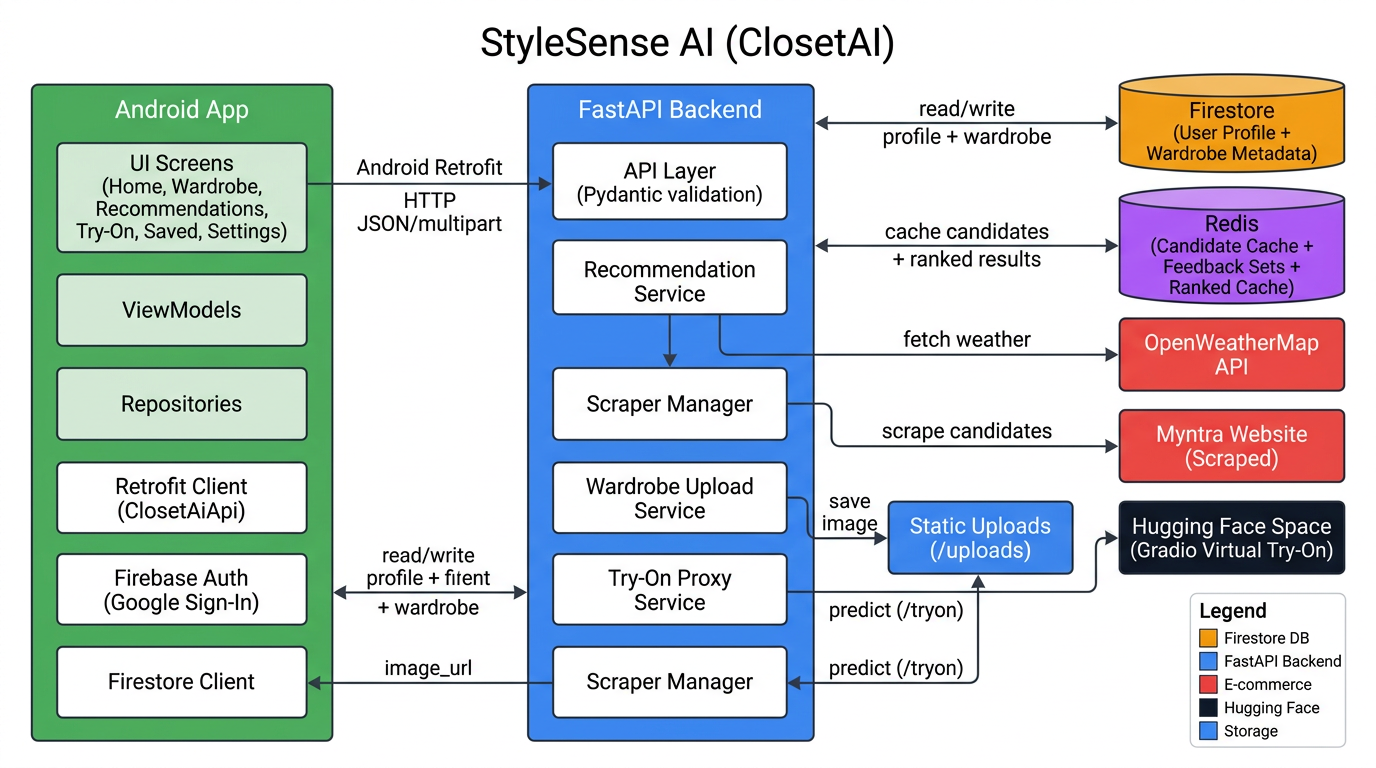
\includegraphics[width=\textwidth]{figures/fig1_system_architecture.png}
\caption{System Architecture of \ProjectShort{}}
\label{fig:architecture}
\end{figure}

\FloatBarrier

\textbf{Figure~\ref{fig:recflow}} shows the recommendation flow from the Android app's Home screen to a ranked product list displayed in the UI.

\begin{figure}[H]
\centering
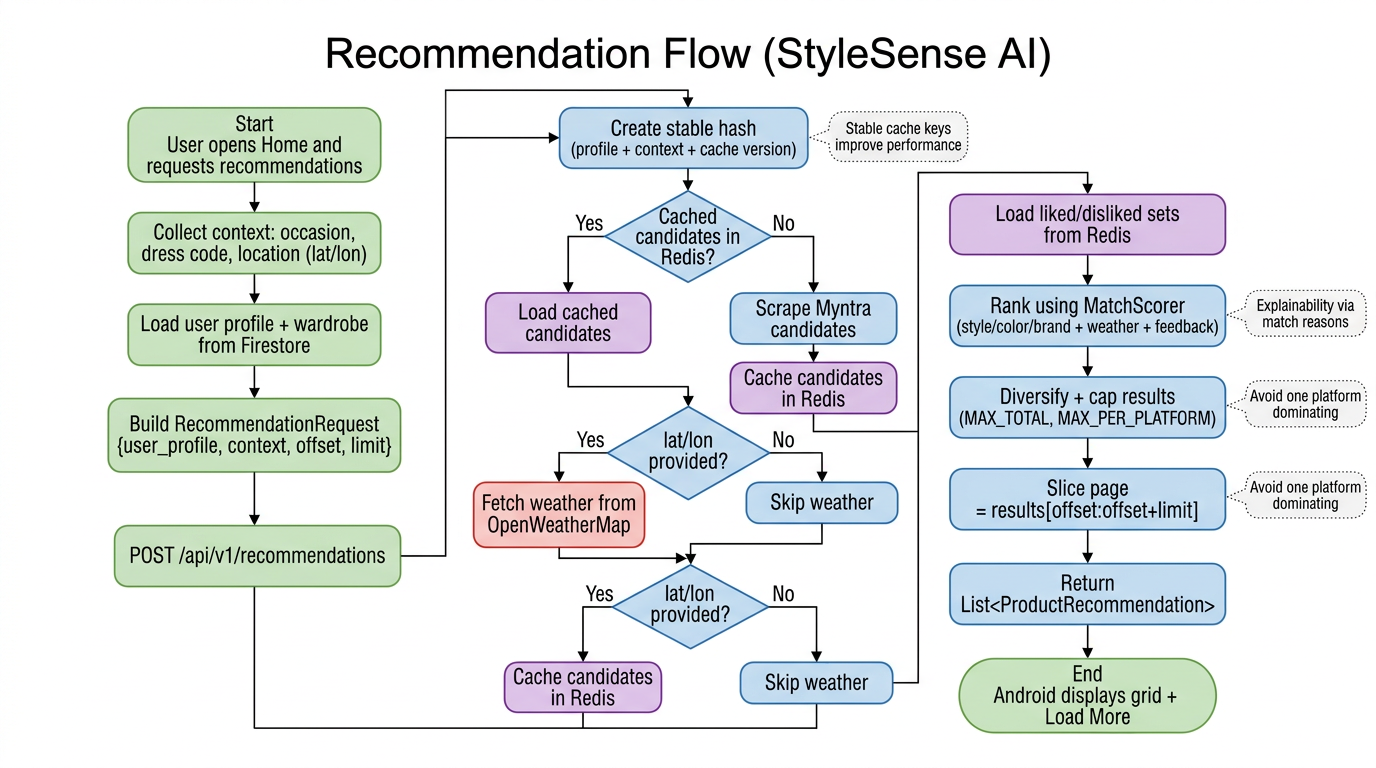
\includegraphics[width=\textwidth]{figures/fig2_recommendation_flow.png}
\caption{Recommendation Flow: Android $\rightarrow$ Backend $\rightarrow$ Ranking $\rightarrow$ UI}
\label{fig:recflow}
\end{figure}

\FloatBarrier

\textbf{Figure~\ref{fig:tryonflow}} shows the virtual try-on flow, from garment selection on Android through backend inference to the displayed result.

\begin{figure}[H]
\centering
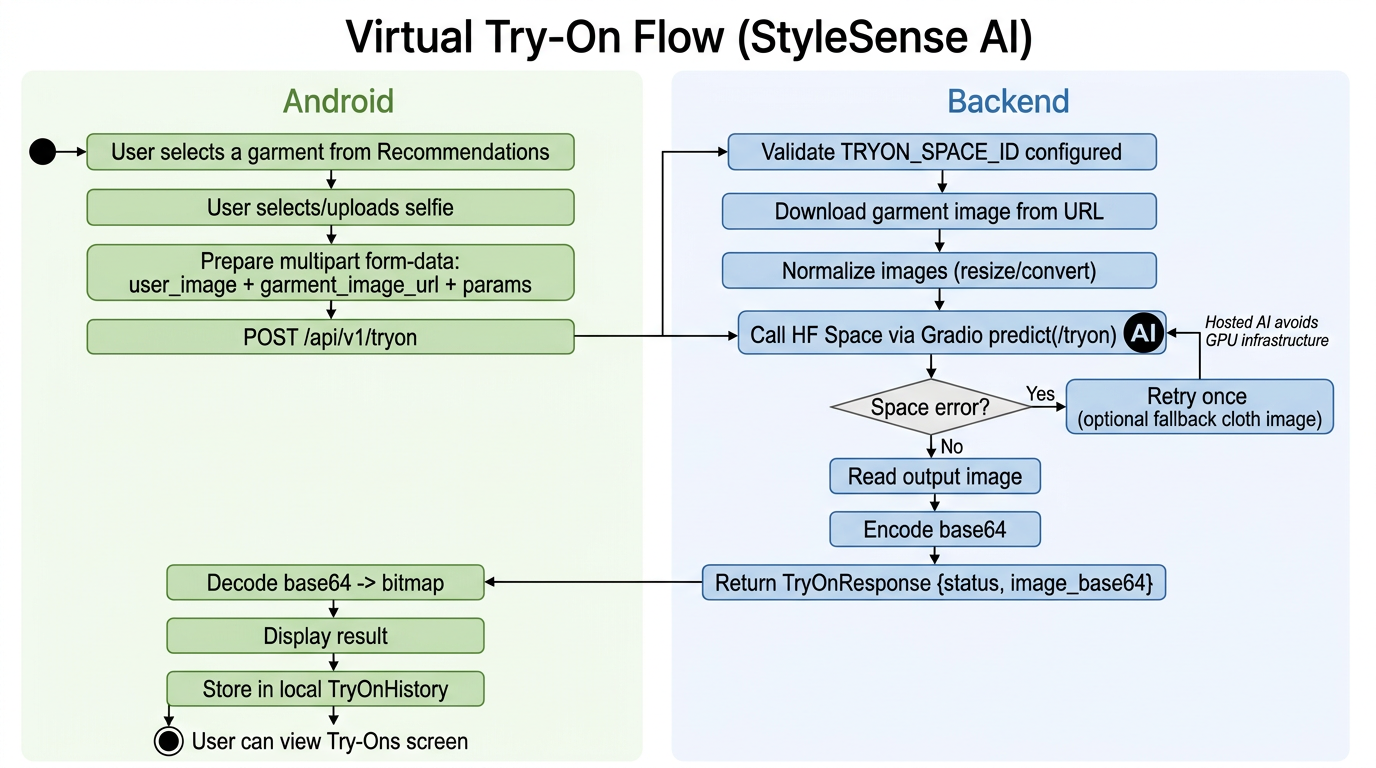
\includegraphics[width=\textwidth]{figures/fig3_tryon_flow.png}
\caption{Virtual Try-On Flow: App Request $\rightarrow$ Backend $\rightarrow$ HF Space $\rightarrow$ Base64 Image}
\label{fig:tryonflow}
\end{figure}

\FloatBarrier

\subsection*{Module Breakdown}

The system is composed of six loosely-coupled modules:
\begin{itemize}
  \item \textbf{Authentication Module:} Manages Google sign-in via Firebase and provides a stable UID used as a primary key across Firestore and Redis.
  \item \textbf{Onboarding Module:} 10-step sequential screen flow that collects profile signals; saves them to Firestore on completion.
  \item \textbf{Wardrobe Module:} Allows users to photograph or pick clothing items, upload them to the backend, and maintain a Firestore-backed wardrobe inventory.
  \item \textbf{Recommendation Module:} Combines Firestore profile, context inputs, live scraping, Redis caching, weather data, and feedback to return a ranked, paginated product list.
  \item \textbf{Try-On Module:} Accepts a user selfie and a garment image URL, routes them through the FastAPI proxy to a hosted AI model, and returns a rendered try-on image.
  \item \textbf{Feedback Module:} Captures like/dislike events, stores them in Redis keyed by UID, and uses them to adjust the next ranking call without re-scraping.
\end{itemize}

\section{Design Selection}

\textit{This section explains the ``why behind each major technology choice in plain terms, suitable for a viva explanation.}

\textbf{Jetpack Compose over XML layouts:} Compose uses a declarative, state-driven model where the UI is a pure function of state. This eliminates the error-prone imperative view manipulation of XML layouts, makes navigation cleaner, and significantly reduces boilerplate code for 12+ screens.

\textbf{FastAPI over Flask:} FastAPI is built on Starlette (async) and Pydantic. This means (i) concurrent scraping tasks can run without blocking the main thread, (ii) request/response payloads are automatically validated against typed models, and (iii) interactive API documentation is generated automatically at \texttt{/docs} --- useful for team coordination.

\textbf{Firebase / Firestore over a custom database:} A custom SQL or NoSQL server would require additional infrastructure (hosting, backups, auth). Firebase is fully managed, free for minor-project scale, supports Google Sign-In natively, and integrates directly with the Android SDK.

\textbf{Hugging Face Space over self-hosted try-on:} Running a VITON-style model locally requires a modern GPU (8--16 GB VRAM) and significant setup. A hosted Space provides free GPU compute through Hugging Face's zero-GPU programme, and the Gradio client library makes invocation straightforward.

\section{Implementation Plan / Methodology}

An \textbf{iterative, module-first methodology} was followed:
\begin{enumerate}
  \item Define API contracts (Pydantic request/response models and Retrofit interfaces) before implementation, so Android and backend can develop in parallel.
  \item Build each backend endpoint with a stub that returns hardcoded data; test with Android before implementing real logic.
  \item Add real logic incrementally: scraper, then MatchScorer, then Redis caching, then weather, then try-on.
  \item For Android, build one screen at a time: sign-in $\to$ onboarding $\to$ home $\to$ recommendations $\to$ wardrobe $\to$ try-on $\to$ saved.
  \item Each sprint ends with a cross-module integration test (Android calls real backend; backend calls real scraper and real Redis).
\end{enumerate}

% =========================================================
% CHAPTER 4 — RESULTS ANALYSIS AND VALIDATION
% =========================================================
\chapter{RESULTS ANALYSIS AND VALIDATION}

\textit{This chapter presents the implementation outcome for each module and validates the end-to-end system. For each module, the implementation is described, the relevant flowchart is shown, and any measurable results are reported. Where exact measurements are environment-dependent, the expected behaviour is described.}

\section{Implementation of Solution}

\subsection{Onboarding Module}

\textbf{Purpose:} Collect all profile signals needed for personalized recommendations from a new user who has no purchase history (cold-start solution).

\textbf{Implementation:} The onboarding consists of 10 sequential Compose screens driven by \texttt{OnboardingViewModel}. Each screen collects one category of information: gender, body type, size measurements, skin tone, style preferences, fit preferences, typical occasions, budget range, special requirements (e.g., plus-size, modest wear), and preferred clothing categories. On completion, the full profile is written as a single Firestore document under \texttt{users/\{uid\}}.

\textbf{Why this matters:} Without onboarding, the backend's MatchScorer would have no profile signals to work with and could only return popularity-sorted items --- effectively the same as any generic e-commerce search. The onboarding data directly feeds the scoring weights.

\begin{figure}[H]
\centering
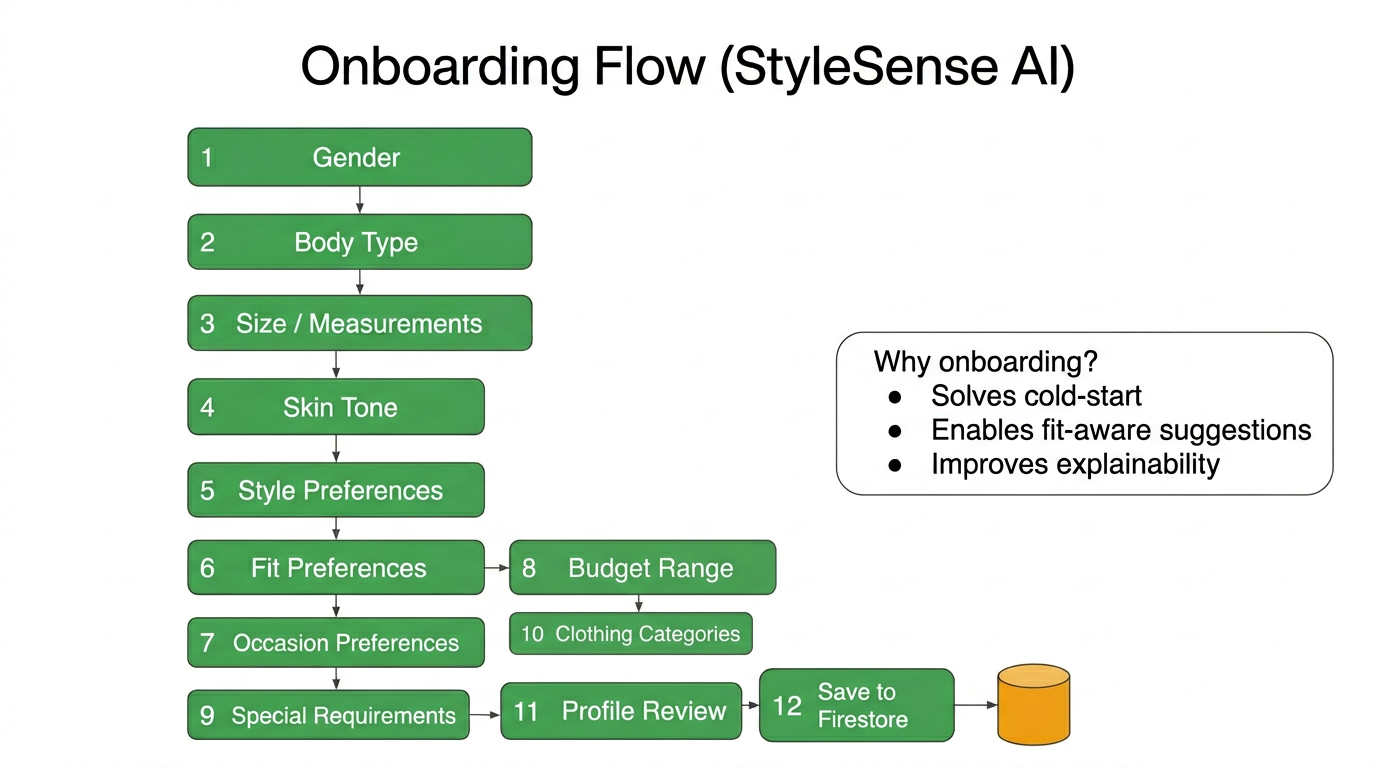
\includegraphics[width=0.88\textwidth]{figures/fig4_onboarding_flow.png}
\caption{Onboarding Screen Flow (10 steps $\rightarrow$ Firestore save)}
\label{fig:onboarding}
\end{figure}

\FloatBarrier

\subsection{Authentication Module}

\textbf{Purpose:} Establish a secure, verified user identity that links the Android app, Firestore data, and backend Redis feedback.

\textbf{Implementation:} Google Sign-In is implemented using Android's Credential Manager API, which presents a bottom sheet for account selection without leaving the app. Firebase Auth processes the credential and returns a UID. A listener on \texttt{SplashScreen} checks whether the user is already signed in (skip onboarding) or is new (route to onboarding). The UID is included in every recommendation and feedback API request so the backend can retrieve the correct Redis feedback sets.

\subsection{Wardrobe Module}

\textbf{Purpose:} Allow users to build a digital inventory of their existing clothes so that recommendations can factor in wardrobe compatibility.

\textbf{Implementation:} The Wardrobe screen shows a grid of owned items loaded from Firestore (ordered by \texttt{addedAt}). A floating action button opens a dialog for image selection (camera or gallery) and metadata entry (category and colour). The image is POSTed as multipart to \texttt{/api/v1/wardrobe/upload}; the backend saves it under \texttt{uploads/wardrobe/} and returns a public URL. The app creates a \texttt{WardrobeItem} document in Firestore with the URL and metadata. On the next recommendation request, wardrobe items are included in the profile payload for the MatchScorer.

\begin{figure}[H]
\centering
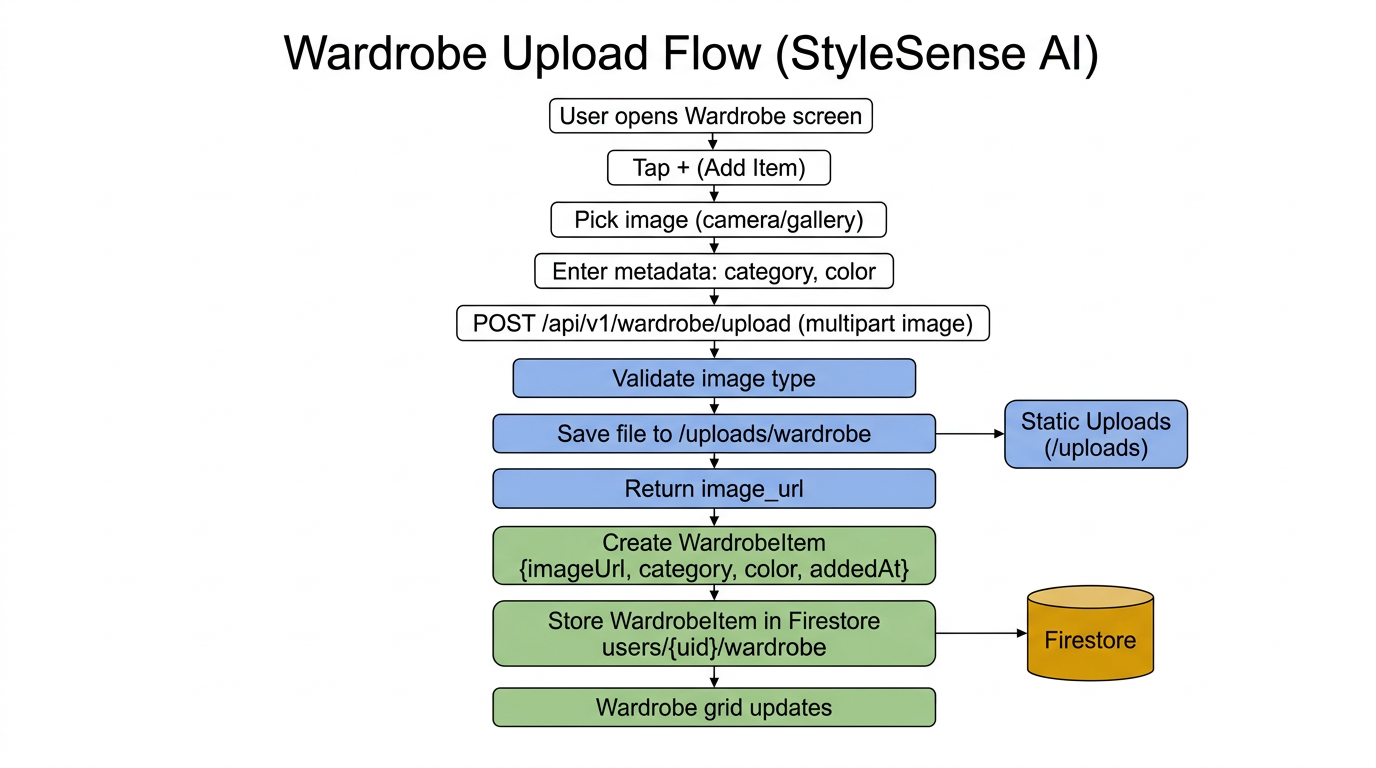
\includegraphics[width=0.88\textwidth]{figures/fig5_wardrobe_upload_flow.png}
\caption{Wardrobe Upload Flow: Android $\rightarrow$ Backend $\rightarrow$ Firestore}
\label{fig:wardrobe}
\end{figure}

\FloatBarrier

\subsection{Recommendation Module}

\textbf{Purpose:} Return a ranked, paginated list of real products from Myntra that match the user's profile and context as closely as possible.

\textbf{Implementation:} \texttt{RecommendationsViewModel} assembles a \texttt{RecommendationRequest} containing the Firestore user profile (including wardrobe), contextual fields from the Home screen (occasion, dress code), and GPS coordinates for weather. The backend:
\begin{enumerate}
  \item Generates a stable MD5 hash of the profile + context to use as a Redis cache key.
  \item If a cached candidate list exists, it is loaded; otherwise Myntra is scraped and the result is cached.
  \item If GPS coordinates are present, the current weather is fetched from OpenWeatherMap.
  \item \texttt{MatchScorer.rank\_products()} scores each candidate by computing keyword overlap on style/colour/brand fields, applying weather adjustments (e.g., boost lightweight fabrics in hot weather), and nudging liked items up / disliked items down.
  \item Results are diversified (capped per platform) and the requested page slice is returned.
\end{enumerate}

\begin{figure}[H]
\centering
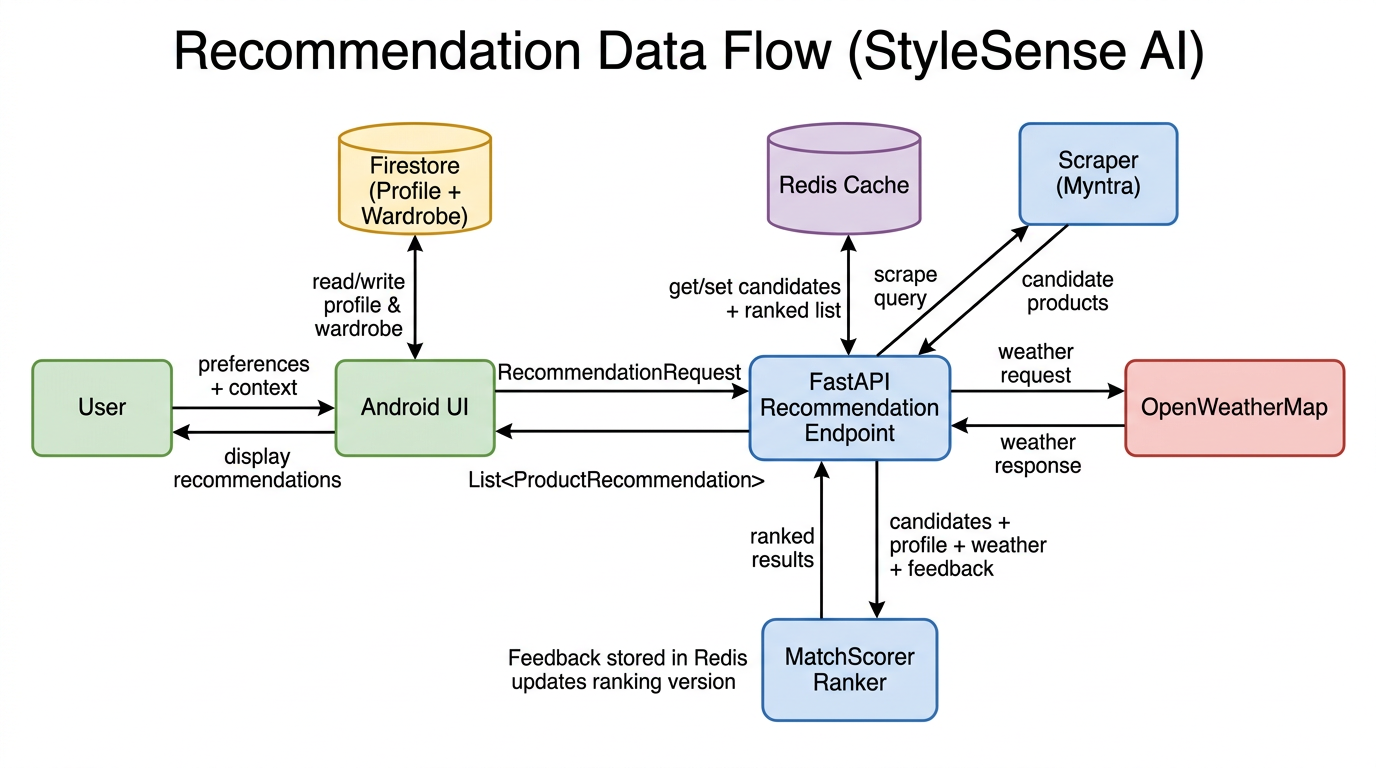
\includegraphics[width=0.88\textwidth]{figures/fig6_recommendation_dataflow.png}
\caption{Recommendation Data Flow (DFD Level 1)}
\label{fig:recdata}
\end{figure}

\FloatBarrier

\subsection{Virtual Try-On Module}

\textbf{Purpose:} Allow users to preview how a recommended garment looks on their own body before deciding to purchase, increasing purchase confidence and reducing returns.

\textbf{Implementation:} From the Recommendations screen, the user taps a ``Try On'' button on any product card. The app loads the stored user selfie (from \texttt{TryOnUserImageStore}) or prompts for one. A multipart POST is sent to \texttt{/api/v1/tryon} containing the selfie and the garment's image URL. The backend downloads and normalises both images, then calls the Hugging Face Space via \texttt{gradio\_client.predict()}. If the Space returns a runtime error (common with scraped garment photos), the backend retries once with a known-good fallback cloth image. The generated output is returned as base64 PNG, decoded by the app, displayed full-screen, and appended to the local \texttt{TryOnHistoryStore} for the Try-Ons screen.

\begin{figure}[H]
\centering
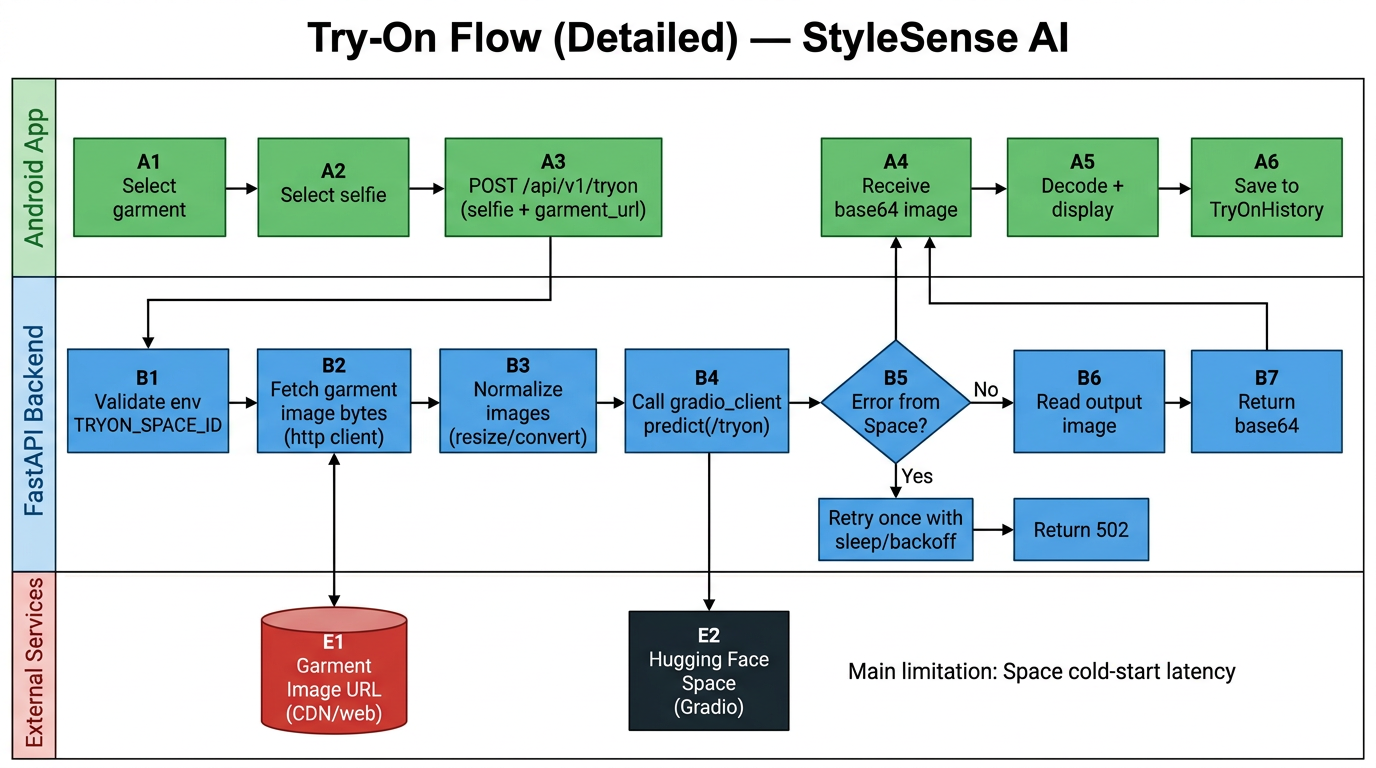
\includegraphics[width=0.88\textwidth]{figures/fig7_tryon_flow_detailed.png}
\caption{Try-On Flow (Detailed Swimlane)}
\label{fig:tryondetail}
\end{figure}

\FloatBarrier

\subsection{Feedback and Saved Items Module}

\textbf{Purpose:} Create a feedback loop so that user preferences improve recommendations over time without requiring a full re-scrape.

\textbf{Implementation:} When a user taps Like or Dislike on a recommendation card, the app POSTs to \texttt{/api/v1/recommendations/feedback}. The backend stores the product ID in a Redis set keyed to the user's UID (liked set or disliked set) and increments a feedback version counter. On the next recommendation request, the ranked-list cache key includes the feedback version, so a changed version triggers a fresh re-ranking run (with nudged scores) while still reusing the cached scraped candidates. Liked items also have their snapshot (title, brand, image URL, price) stored in a Redis hash for retrieval by the Saved screen via \texttt{GET /api/v1/recommendations/saved/\{uid\}}.

\subsection{Quantitative Summary}

\textit{Table~\ref{tab:endpoints} summarises each backend endpoint, its output, and its validated behaviour. Response times are indicative; actual times depend on network conditions, Redis availability, and Hugging Face Space load.}

\vspace{4pt}
\begin{table}[H]
\centering
\caption{Backend Endpoint Validation Summary}
\label{tab:endpoints}
\begin{adjustbox}{max width=\linewidth}
\small
\begin{tabular}{L{0.32\linewidth} L{0.10\linewidth} L{0.17\linewidth} L{0.34\linewidth}}
\toprule
\textbf{Endpoint} & \textbf{Method} & \textbf{Approx.\ Time} & \textbf{Validated Behaviour} \\
\midrule
{\ttfamily /health}
  & GET & $<$100 ms & Returns environment and status; confirms backend reachability from Android Settings. \\
{\ttfamily /api/v1/wardrobe/ upload}
  & POST & 200--500 ms & Saves image to disk; returns public \texttt{image\_url} via \texttt{/uploads}. \\
{\ttfamily /api/v1/ recommendations}
  & POST & 2--8 s; $<$500 ms (cached) & Ranked + diversified product page; Redis cache dramatically reduces repeat latency. \\
{\ttfamily /api/v1/ recommendations/ feedback}
  & POST & $<$200 ms & Stores liked/disliked IDs in Redis; increments feedback version for re-ranking. \\
{\ttfamily /api/v1/ recommendations/ saved/\{uid\}}
  & GET & $<$300 ms & Returns all liked item snapshots for the Saved screen. \\
{\ttfamily /api/v1/tryon}
  & POST & 20--60 s & Calls HF Space via Gradio; returns base64 image. Latency dominated by Space cold-start. \\
{\ttfamily /api/v1/scrapers/ connectivity}
  & GET & 3--10 s & Probes Myntra reachability; diagnoses zero-result scraping failures. \\
\bottomrule
\end{tabular}
\end{adjustbox}
\end{table}

% =========================================================
% CHAPTER 5 — CONCLUSION AND FUTURE WORK
% =========================================================
\chapter{CONCLUSION AND FUTURE WORK}

\section{Conclusion}

\ProjectShort{} successfully demonstrates a full-stack, context-aware fashion assistant that goes beyond the capability of existing commercial apps available to Indian consumers. The system covers the complete user journey: onboarding for cold-start personalization, a digital wardrobe for compatibility awareness, live product recommendations scored by a multi-factor engine, weather-aware ranking through GPS and OpenWeatherMap integration, a feedback loop that improves results over time, and AI-based virtual try-on through a hosted model.

From an engineering perspective, the project achieves a working integration of six distinct technologies (Android/Compose, FastAPI, Firebase, Redis, OpenWeatherMap, Hugging Face Spaces) within the constraints of a minor project: no GPU infrastructure, no large training dataset, and no paid cloud services. Each design decision --- rule-based scoring, hosted try-on, Redis caching with fallback, static image storage --- was directly motivated by these constraints and validated in implementation.

The project demonstrates that meaningful AI-assisted personalization is achievable without training custom models, by combining well-chosen APIs, an explicit user profile, and a thoughtfully designed scoring function.

\section{Future Work}

The following improvements are planned or recommended for a follow-up major project or production deployment:

\begin{itemize}
  \item \textbf{Multi-store scraping:} Expand data collection to AJIO, Amazon Fashion, and H\&M, and build a scraper manager that merges and deduplicates candidates across sources.
  \item \textbf{Learning-based ranking:} Replace the rule-based MatchScorer with a learned pairwise ranker (e.g., LambdaMART or a small neural ranker) trained on accumulated feedback events.
  \item \textbf{Image-based wardrobe tagging:} Use a garment classification model (deployable as a TFLite model on-device) to automatically tag uploaded wardrobe photos with category, colour, and style --- removing the need for manual metadata entry.
  \item \textbf{Outfit builder:} Leverage outfit compatibility modelling (motivated by Cheng et al., 2021) to suggest complete outfits (top + bottom + footwear) instead of individual items.
  \item \textbf{Try-on quality and latency:} Explore self-hosting a quantized VITON model on a low-cost GPU VM to eliminate HF Space cold-start latency and support batch processing.
  \item \textbf{Offline mode:} Cache the most recent recommendation page and wardrobe inventory on-device so the app remains usable without an internet connection.
\end{itemize}

% =========================================================
% REFERENCES
% =========================================================
\begin{thebibliography}{99}
\addcontentsline{toc}{chapter}{REFERENCES}

\bibitem{deepfashion}
Liu, Z., Luo, P., Qiu, S., Wang, X., \& Tang, X. (2016).
DeepFashion: Powering Robust Clothes Recognition and Retrieval with Rich Annotations.
\textit{Proceedings of the IEEE Conference on Computer Vision and Pattern Recognition (CVPR)}, pp.\ 1096--1104.

\bibitem{resnet}
He, K., Zhang, X., Ren, S., \& Sun, J. (2016).
Deep Residual Learning for Image Recognition.
\textit{Proceedings of the IEEE Conference on Computer Vision and Pattern Recognition (CVPR)}, pp.\ 770--778.

\bibitem{viton}
Han, X., Wu, Z., Wu, Z., Yu, R., \& Davis, L. S. (2018).
VITON: An Image-based Virtual Try-on Network.
\textit{Proceedings of the IEEE Conference on Computer Vision and Pattern Recognition (CVPR)}, pp.\ 7543--7552.

\bibitem{contextrecsys}
Adomavicius, G., \& Tuzhilin, A. (2011).
Context-Aware Recommender Systems.
In F. Ricci et al.\ (Eds.), \textit{Recommender Systems Handbook}, pp.\ 217--253. Springer.

\bibitem{outfitcompat}
Cheng, Z., et al.\ (2021).
Learning Outfit Compatibility with Graph Neural Networks.
\textit{ACM Transactions on Information Systems}.

\bibitem{linden2003}
Linden, G., Smith, B., \& York, J. (2003).
Amazon.com Recommendations: Item-to-Item Collaborative Filtering.
\textit{IEEE Internet Computing}, 7(1), 76--80.

\bibitem{fastapi}
Ramírez, S. (2024). FastAPI Documentation. \url{https://fastapi.tiangolo.com/}

\bibitem{compose}
Google. (2024). Android Jetpack Compose Documentation. \url{https://developer.android.com/compose}

\bibitem{firebase}
Google. (2024). Firebase Authentication Documentation. \url{https://firebase.google.com/docs/auth}

\bibitem{openweather}
OpenWeather Ltd. (2024). OpenWeatherMap API Documentation. \url{https://openweathermap.org/api}

\end{thebibliography}

% =========================================================
% APPENDIX
% =========================================================
\appendix

\chapter{Plagiarism Report}

Attach the plagiarism report generated by your institute's approved tool (e.g., Turnitin, iThenticate, Urkund). The report should show a similarity index below the acceptable threshold set by your department.

\chapter{Design Checklist}

\textit{This checklist confirms that all major engineering and design steps were completed before submission.}

\vspace{4pt}
\begin{table}[H]
\centering
\caption{Design and Implementation Checklist}
\begin{adjustbox}{max width=\linewidth}
\begin{tabular}{L{0.66\linewidth} L{0.20\linewidth}}
\toprule
\textbf{Checklist Item} & \textbf{Status} \\
\midrule
Requirements identified and mapped to modules & Completed \\
API contracts defined (Pydantic models + Retrofit interfaces) & Completed \\
UI navigation graph and screen flow verified & Completed \\
Backend endpoints implemented and tested individually & Completed \\
Scraper produces valid product candidates for test queries & Completed \\
Redis caching and in-memory fallback behaviour confirmed & Completed \\
Firebase Auth sign-in and Firestore read/write tested & Completed \\
Virtual try-on integration tested with sample selfie and garment image & Completed \\
Feedback like/dislike updates Redis and changes ranking & Completed \\
Saved items endpoint returns correct liked snapshots & Completed \\
\bottomrule
\end{tabular}
\end{adjustbox}
\end{table}

\chapter{User Manual}

\section{System Requirements}

\begin{itemize}
  \item Android device or emulator running Android 8.0 (API 26) or higher.
  \item The FastAPI backend running on a host reachable from the device (local network or public server).
  \item Active internet connection for scraping, weather, and try-on.
  \item Redis running locally or on the same host as the backend (optional but recommended).
\end{itemize}

\section{Backend Setup}

\begin{enumerate}
  \item Navigate to the \texttt{backend/} directory.
  \item Create a \texttt{.env} file and set \texttt{TRYON\_SPACE\_ID}, \texttt{HF\_TOKEN} (optional), and \texttt{OPENWEATHER\_API\_KEY}.
  \item Install dependencies: \texttt{pip install -r requirements.txt}
  \item Start the server: \texttt{uvicorn main:app --host 0.0.0.0 --port 8081 --reload}
\end{enumerate}

\section{Android App Setup}

\begin{enumerate}
  \item Open the \texttt{closetai/} directory in Android Studio.
  \item Place your \texttt{google-services.json} in \texttt{app/}.
  \item Build and run on an emulator or physical device.
  \item On first launch, open the Settings screen and set the backend base URL (emulator default: \texttt{http://10.0.2.2:8081/}).
\end{enumerate}

\section{How to Use the Application}

\begin{enumerate}
  \item \textbf{Sign in:} Tap ``Sign in with Google'' and select your Google account.
  \item \textbf{Complete onboarding:} Fill in all 10 profile steps. You can change these later via Settings.
  \item \textbf{Add wardrobe items:} Open the Wardrobe tab, tap \textbf{+}, pick an image, enter category and colour, and tap Save.
  \item \textbf{Get recommendations:} On the Home screen, select occasion and dress code, then tap ``Get Recommendations''. Allow location for weather-aware results.
  \item \textbf{Like / Dislike items:} Tap the thumbs-up or thumbs-down icon on any recommendation card. Liked items appear in the Saved tab.
  \item \textbf{Try On:} Tap ``Try On'' on a product card. If no selfie is stored, you will be prompted to take one. The generated try-on image is displayed and saved to Try-Ons history.
\end{enumerate}

\end{document}
